% Introdu��o
\chapter{Introduction}

The goal of this chapter is to present the technical concepts for a better understanding of our job. 


\section{Cloud Computing \& The technological shift}

The adoption of cloud solutions is growing fast among organizations~\cite{6546068}.
Centralized (mostly mainframe) technology is being replaced by distributed and more flexible forms of data storage and processing.
This change of paradigm is motivated by the necessity to improve the use of resources, as well as by the increasing velocity in which data is produced.

In this scenario, transitions must take into account the quality of the service delivered by the new solutions.

On the early 90's it was commonplace for every Information Technology (IT) company to have its own Data Center with huge servers and mainframes. 
IT costs were high, and high-performance computing was available only for big companies, as data centers required a large physical infrastructure and have high costs for maintenance~\cite{Armbrust09m.:above}.

The regular way of building a web application was to use a client-server approach, where the server was a powerful (and expensive) machine. 
At the same time, new players, such as Google or Yahoo, were rising with bigger missions: \textit{``to organize the world's information and make it universally accessible and useful''}~\cite{Spector:2012:GHA:2209249.2209262}. 
The popularization of the internet use incentivized new ways of commerce exchange, yielding an explosion in the amount of data produced and exchanged. 
It was \textit{just} impossible to store the petabytes of daily-generated data in a single server. 

From this point on, the community realized the economical convenience of building and maintaining several low-performance servers, instead of a single high-performance one, even if this this requires a change of culture in the administration of the new datacentres.
The new approach is also incompatible with the traditional way of building applications, that usually were designed to work on a single server and database. 

Several research initiatives were conducted in this area and a common solution was rising: to distribute data storage and processing. 
Google, Yahoo and other big IT players helped to build open source tools to make this approach possible, like Hadoop~\cite{5496972}.

This revolution brought to life the notion of \textit{Cloud Computing}, together with new concepts, such as Infrastructure as a Service \textit{(IAAS)}, Platform as a Service \textit{(PAAS)} and Software as a Service \textit{(SAAS)}~\cite{AViewOfCloudComputing}.
According to~\cite{AViewOfCloudComputing}, \textit{Cloud computing refers to both the applications delivered as services over the Internet and the hardware and systems software in the data centers that provide those services.} 


\section{Data Integration \& Polyglot Persistence}
On the last years, the number of Data Base (DB) Engines grew like never before~\cite{dbranking}. 
Along with the NoSQL (Not only SQL) movement and expansion of Social Networks, new concepts for Database Models appeared, like Document Store, Search Engines, Key-Value store, Wide Column Store, Multi-Model and Graph DBMS. 
In~\cite{dbranking} a ranking of the most popular DB engines is presented.

Today, instead of having a single Relational Database Management System (DBMS) for the whole application, it is efficient and cost-effective to have several Data Base Engines, one for each type of data that the application handles. 
This concept is called \textit{Polyglot Persistence}~\cite{sadalage2012nosql}.

As \cite{AdressingDataManagementCloud} illustrates, polyglot persistence is very useful in the context of  e-commerce applications that deal with a catalog, user access logs, financial information, shopping carts and purchase transactions, for example.
The notion of polyglot persistence is built upon the observation that the \textit{nature} of each data type is significantly different (i.e: user logs imply high volume of writes on multiple nodes, shopping carts need high availability and user sessions require rapid access for reads and writes). 

As computing services started to decentralize, developers started to build applications that depended of several data-sources. 
By this time the use of Web Services and Service Oriented Architecture (SOA) became more popular~\cite{Armbrust09m.:above}. 


\section{Systematic Mappings}
According to \cite{Petersen:2008:SMS:2227115.2227123}, ``\textit{A software engineering systematic map is a defined method to build a classification scheme and structure a software engineering field of interest.}''
Systematic Mapping studies provide a global view of a given research field and identify the quantity, results, and the kinds of researches in this field.

A Systematic map is composed by a number of steps (Figure~\ref{fig:sms}).
\begin{figure}[ht!]
\centering
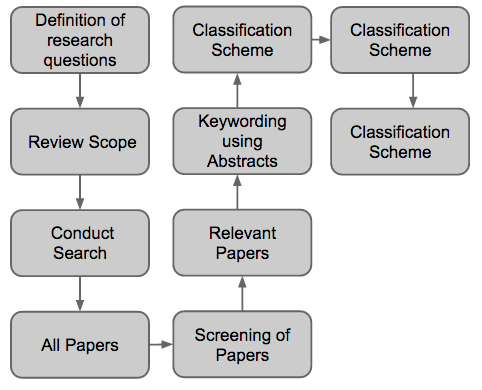
\includegraphics[width=100mm]{Imagens/pic1.png}
\caption{Systematic Mapping Steps~\cite{Petersen:2008:SMS:2227115.2227123}.\label{fig:sms}}
\end{figure}

On the first step, ``Definition of Research question'', the questions that must be answered on the survey are defined. 
On the ``Review Scope'' step, researchers target the papers/journal sources that will be taken into consideration on the systematic map. 
After that, the ``Search'' step is done using a set of predefined search engines and a body of papers (``All papers'') is retrieved. 

After an initial ``Screening of the papers'', the ``Relevant papers'' are chosen according to inclusion and exclusion criteria defined by the research team. 
At this point, the papers that will participate of the study are selected. 
The selection is based on the title, abstracts and keywords of each paper (``Keywording using Abstracts'').

After that, a ``Classification Scheme'' is built, defining different points-of-view (or facets) from which the body of papers will be classified. 
After matching each paper with the classification schema (``Data Extraction and Mapping Process''), the  systematic mapping is performed.
In this phase the relationships between the collected data (in the light of the classification scheme) are used to answer the research questions.


\section{Service Level Agreements (SLAs)}
According to \textit{ITILv3's} official glossary \cite{itilv3glossary}, a Service Level Agreement (SLA) is ``\textit{an agreement between an IT service provider and a customer. 
A service level agreement describes the IT service, documents service level targets, and specifies the responsibilities of the IT service provider and the customer.}'' 

The agreement consists on a set of measurable constraints that a service provider must guarantee to its customers.
In practical terms, it is a document that a service provider delivers to its consumers with minimum quality of service (QoS) metrics. 
If the service is delivered with a lower QoS than is promised on the SLA, consumers may be refunded or earn benefits that were accorded beforehand.    